\documentclass[a4paper, 12pt, svgnames]{article}

\usepackage{preambule}

\title{Variabilités intrinsèques des SNe Ia et leurs conséquences sur les
paramètres cosmologiques}

\fancyhead[L]{\scriptsize \textsc{Variabilités intrinsèques des SNe Ia}}

\begin{document}

\thispagestyle{empty}
\noindent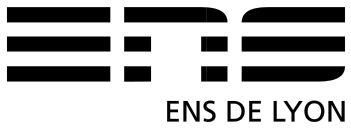
\includegraphics[height=2cm]{General_figures/logoens.png} \hfill

\includegraphics[height=2cm]{General_figures/logoucbl.png} \hfill

\includegraphics[height=2cm]{General_figures/logounivlyon.png}\vfill

\noindent\begin{tabularx}{\linewidth+27pt}{@{} l X r @{} }
{\textsc{Master Science de la matière}} & & Année 2018--2019\hspace*{1cm}\\
{\textit{École Normale Supérieure de Lyon}} & & \textsc{Nicolas} Nora\hspace*{1cm}\\
{\textit{Université Claude Bernard Lyon I}} & & M2 Physique\hspace*{1cm}
\end{tabularx}

\begin{center}\vfill\hrule\vspace*{8pt}

\textbf{\huge Variabilités intrinsèques des SNe Ia et leurs conséquences sur les
paramètres cosmologiques}\\

\hrule\vfill

\parbox{15cm}{\small\textbf{Résumé}:
L'étude des supernovae de type Ia a de nombreuses utilités en physique. Elle
sert notamment à la détermination de paramètres cosmologiques, comme la
constante de Hubble ou le paramètre d'état de l'énergie noire. Afin d'améliorer
la précision et la justesse des mesures existantes, les incertitudes
statistiques et systématiques doivent être traitées correctement. Si l'ajout de
données permet de réduire les incertitudes statistiques, il n'y a que l'étude du
comportement physique des supernovae qui permet de réduire les incertitudes
systématiques. Dans ce rapport, nous discutons comment l'établissement de lois
d'évolution du paramètre de durée d'explosion d'une supernova en fonction du
redshift permettrait d'atteindre ce but.}\vspace{0.5cm}

\parbox{15cm}{\small\textbf{Mots-clés}:
Cosmologie, supernovae}\vspace{0.5cm}

\parbox{15cm}{Stage supervisé par:\\
\textbf{\textsc{RIGAULT} Mickaël}, Chercheur\\
\href{mailto:rigault@ipnl.in2p3.fr}{rigault@ipnl.in2p3.fr}\\
\href{https://www.ipnl.in2p3.fr/perso/rigault/}{Site personnel}\bigbreak
Institut de Physique des Deux Infinis\\
{\textit{Université Lyon 1\\4 rue Enrico Fermi -- bâtiment Dirac\\
69622 Villeurbanne Cedex}}\\
\url{https://www.ipnl.in2p3.fr}}\vspace{.5cm}\vfill


\includegraphics[width=.3\textwidth]{General_figures/IP2I.png}
\end{center}\vfill \hfill \today
\newpage
\thispagestyle{empty}
\setcounter{page}{0}

\appsec{Remerciements}{sec:ack}

Je tiens à remercier toutes les personnes qui ont contribué, de près ou de loin,
à la réalisation de ce stage et de ce rapport de stage. En premier lieu, bien
évidemment, je remercie Mickaël \bsc{Rigault} pour son encadrement sans faille

\tableofcontents
\newpage

\section{Introduction}\label{sec:int}
\subsection{Le domaine de recherche}

La combinaison des observations et des prédictions théoriques du modèle du Big
Band indiquent que l'univers est en expansion. Lors de la découverte de cette
expansion, on pensait qu'elle devrait ralentir sous l'effet de la gravitation.
Cependant, l'utilisation des supernovae de type Ia (SNe Ia) par \bsc{Perlmutter
et al.}~\cite{perlmutter_measurements_1999}, \bsc{Riess et al.}
~\cite{riess_observational_1998} et \bsc{Schmidt et al.}
~\cite{schmidt_high-z_1998} a permis de mettre en évidence l'expansion
accélérée de l'Univers, découverte pour laquelle ils ont eu le prix Nobel de
physique de 2011. Il y aurait ainsi un phénomène allant à l'encontre des
effets gravitationnels, phénomène qui a été nommé « énergie noire » : la
cosmologie moderne vise entre aux à mieux comprendre la nature de cette énergie,
sa proportion dans l'Univers et les lois physiques auxquelles elle obéit.

\begin{itemize}
    \item Tension sur $H_0$? \bsc{Riess et al.} 2016 donne des valeurs en intro
\end{itemize}

\subsection{Diagramme de Hubble}
Cette découverte a été effectuée par l'utilisation des mesures des flux lumineux
de supernovae, exprimés en magnitude qui en est le logarithme. Le flux est relié
à la luminosité $L$ d'une source lumineuse et à la distance $d_L$ entre la source
et le point d'observation par la relation

\begin{equation}
    F = \frac{L}{4\pi d_L²}
\end{equation}

et la magnitude apparente $m$ est reliée au flux reçu par la relation

\begin{equation}
    m - m_0 = -2.5\log\LR{F}{F_0} = -2.5\log\LR{L}{4\pi d_L²} + C
\end{equation}

avec $F_0$ le flux d'une étoile de référence. Cette définition de la magnitude
dépend donc de la distance ; on définit alors une magnitude \textit{absolue}
traduisant la luminosité intrinsèque du corps observé : c'est la magnitude
apparente que percevrait un observateur situé à une distance de $\SI{10}{pc}$ de
la source, autrement dit

\begin{equation}
    M = -2.5\log\LR{L}{4\pi\LF{\SI{10}{pc}}²} + C
\end{equation}

On peut alors définir le \textit{module de distance} $\m$ défini par

\begin{equation}
    \m \equiv m - M = 5\log(d_L) - 5
\end{equation}

avec $d_L$ en parsec. Or, en considérant un univers plat homogène et isotrope,
l'équation de \bsc{Friedmann}-\bsc{Lemaître} mène à une expression de $d_L$
dépendant des paramètres cosmologiques d'après la relation

\begin{equation}
    d_L = \LF{1 + z} \times c \LF{ \int_0^z \d z' \left[ \O_R
    \LF{1 + z'}⁴ + \O_M \LF{1 + z'}³ + \O_{\L} \right]^{-1/2}}
\end{equation}

\textcolor{orange}{Rajouter développement en annexe ?}

et le module de distance $\m$ permet de de déterminer $d_L$ \textit{via} la
mesure de la magnitude apparente $m$, si la magnitude absolue $M$ est connue.
Les SNe Ia sont utilisées pour leur magnitude absolue \textit{a priori}
standard, ce qui leur a valu le nom de \textit{chandelles standards}.

En réalité, il existe une dispersion naturelle d'environ 40\% des magnitudes
absolues des SNe Ia. Cette dispersion implique une imprécision sur la valeur de
la distance déduite par la mesure de magnitude apparente de 20\%, comme le
montre la figure ci-après :

\begin{figure}[htbp!]
    \centering
    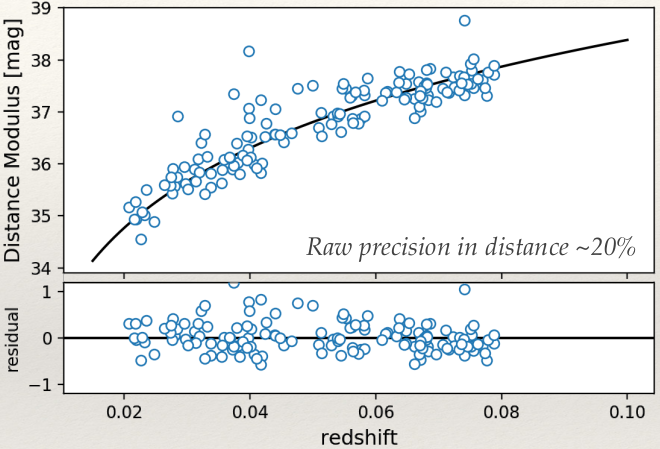
\includegraphics[width = .5\linewidth]{Rapport_figures/disp_40.png}
    \caption{Effet de la dispersion naturelle de la magnitude absolue des SNe Ia
    sur la mesure du module de distance par rapport à l'évolution attendue (en
    noir).}
    \label{disp_40}
\end{figure}

\begin{itemize}
    \item Mesure de magnitude, équations ;
    \item Dispersion naturelle, imprécision.
\end{itemize}

\subsection{Les SNe Ia}
\begin{itemize}
    \item Spécificité astrophysique ;
    \item Pertinence cosmologique.
\end{itemize}

\subsection{Courbes de lumière}
\begin{itemize}
    \item Définitions ;
    \item Relations empiriques, équation corrigée.
\end{itemize}

\subsection{Incertitudes systématiques}
\begin{itemize}
    \item Importance dans les mesures actuelles ;
    \item Importance dans les mesures futures.
\end{itemize}

\subsection{Problème du progéniteur}
\begin{itemize}
    \item Progéniteur inconnus :
    \item L moyennes différentes avec $z$ ou échantillon ;
    \item Évolution du \textit{lsSFR}.
\end{itemize}

Parler du fait que le code est sur GitHub, et faire des références dans la
suite.

\section{Construction d'un échantillon complet}
\subsection{Effets de sélection}
\begin{itemize}
    \item Histogramme échantillons ;
    \item Rappel relation \textcolor{red}{brighter-slower} et conclusion.
\end{itemize}

\subsection{Méthode de détermination}
\begin{itemize}
    \item Modèle d'évolution ;
    \item Statistique poissonienne, itérations pour chaque échantillon.
\end{itemize}

\section{Modèle d'évolution}
\subsection{Origine du modèle}
\begin{itemize}
    \item Données \textcolor{orange}{SNF} ;
    \item Définition jeune/vieille d'après \bsc{Rigault et al.} 2018
\end{itemize}

\subsection{Implémentation aux échantillons}
\begin{itemize}
    \item Concordance avec \textcolor{orange}{SNF} seulement
    \item Modèle \textcolor{orange}{SNF} sur toutes les données
\end{itemize}

\subsection{Modifications et comparaisons}
\begin{itemize}
    \item Modification du modèle ;
    \item Implémentation d'autres modèles et résultats
\end{itemize}

\section{Conclusion}
Conclusion

\bibliographystyle{unsrt}
\bibliography{VIDSTIA}
\addcontentsline{toc}{section}{Bibliographie}

\end{document}
